\documentclass[11pt,letterpaper]{article}
\usepackage[utf8]{inputenc}
\usepackage[T1]{fontenc}
\usepackage{mathptmx}
\usepackage[letterpaper,left=1.25in,right=1.25in,top=1.2in,bottom=1.2in,headheight=14pt]{geometry}
\usepackage{microtype}
\usepackage{amsmath,amssymb,amsthm,mathtools,bm}
\usepackage{graphicx,booktabs,array,multirow,float}
\usepackage{xcolor}
\usepackage{enumitem}
\usepackage[labelfont=bf,labelsep=colon,font=small,skip=4pt]{caption}
\usepackage{subcaption}
\usepackage{fancyhdr}
\usepackage{titlesec}
\usepackage{listings}
\usepackage{tikz}
\usetikzlibrary{arrows.meta,positioning,calc}
\usepackage[authoryear,round]{natbib}
\definecolor{linkcol}{HTML}{2B3A8F}
\usepackage[colorlinks=true,linkcolor=linkcol,citecolor=linkcol,urlcolor=linkcol]{hyperref}
\usepackage[capitalise,noabbrev]{cleveref}

\pagestyle{fancy}\fancyhf{}
\lhead{\small Technical report.}
\cfoot{\small\thepage}
\renewcommand{\headrulewidth}{0.5pt}
\setlength{\parskip}{4pt plus 1pt}\setlength{\parindent}{0pt}
\titleformat{\section}{\large\bfseries}{\thesection}{0.8em}{}
\titleformat{\subsection}{\normalsize\bfseries}{\thesubsection}{0.8em}{}
\titleformat{\subsubsection}{\normalsize\bfseries\itshape}{\thesubsubsection}{0.8em}{}
\titlespacing*{\section}{0pt}{16pt}{6pt}\titlespacing*{\subsection}{0pt}{12pt}{4pt}
\setlist{itemsep=1pt,topsep=3pt}
\setlength{\emergencystretch}{2em}

\theoremstyle{definition}
\newtheorem{definition}{Definition}
\theoremstyle{remark}
\newtheorem{remark}{Remark}

\lstset{basicstyle=\ttfamily\small,breaklines=true,frame=single,framerule=0.3pt,
  xleftmargin=4pt,xrightmargin=4pt,columns=fullflexible,keepspaces=true,showstringspaces=false}

% title block: \reporttitle{title}{subtitle}{authors}{affiliation line}
\newcommand{\reporttitle}[4]{%
\begin{center}
{\LARGE\bfseries #1\\[4pt]
\Large #2\par}
\vspace{1.4em}
{\bfseries\color{linkcol}\large #3}\\[0.4em]
{\small #4}\par
\vspace{1.2em}
\end{center}}
\newcommand{\abstractblock}[1]{%
\begin{center}\textbf{Abstract}\end{center}
\vspace{-0.4em}
\begin{quote}\small #1\end{quote}
\vspace{0.4em}}

\begin{document}
\reporttitle{Harvesting Energy from Traffic-Induced Wind}{A Compact Vertical-Axis Turbine with a Carbon-Fibre Rotor,\\ and the Instrumentation Used to Measure It}{Román I.\,Villarreal \quad Juan Fernando Castaño \quad Larissa Al Kseiri}{Engineering Capstone, New York University Abu Dhabi, May 2025 \quad $\cdot$ \quad Supervisors: P.\,George, J.\,Teo, J.\,I.\,Ryu\\ \href{mailto:jfc9577@nyu.edu}{jfc9577@nyu.edu}}

\abstractblock{Fast highway traffic leaves a turbulent wake that is not harvested. For our engineering capstone we designed, simulated, built and tested a small vertical-axis wind turbine for roadside use in Abu Dhabi, and developed an all-composite carbon-fibre rotor made entirely by hand layup: blades laid up in PLA-printed moulds, a tube wrapped on a mandrel, and a hub plate cut from a flat laminate. The number of plies came from flexural bending tests of coupons and a static finite-element study of the hub, which used loads from our own per-revolution aerodynamic model. In side-by-side logged records the carbon-fibre prototype gave about 3.2 times the mean output voltage of the first PLA prototype (about 6.8\,V against 2.1\,V) and stayed above 2\,V for about 88\% of the record against 42\%. We also built the self-contained data logger (voltage divider, SD card, change-triggered logging) used for all measurements. Flexural tests put hand-laid carbon laminates at about 475--600\,MPa, against 215--395\,MPa for the glass and chopped-strand laminates tested alongside. The records are voltages and not power, and were taken in separate sessions under different wind; load-based power measurement, fatigue, noise and UV and thermal tests remain to be done. Aerodynamic profile definitions, rotor dimensions and laminate schedules are withheld because of an intellectual-property and patent filing.}

\section{Introduction}
Vehicles travelling above 120\,km/h on UAE highways leave wakes in which the air speed reaches about 2.25\,m/s one metre from the lane, the figure we took as our design reference. Conventional wind turbines are designed for steady, high-altitude wind at Reynolds numbers above $10^5$ and are poorly matched to low, turbulent, multi-directional flow near the ground. Roadside space is also restricted, so a candidate has to be compact. The intended use is to power roadside loads such as LED lighting and sensors without a grid connection.

\textbf{Question 1: can a compact vertical-axis turbine produce usable output from traffic-induced wind?} The answer depends on a rotor that starts in weak wind, which means low mass and high stiffness, and on a way of measuring what it produces.

\textbf{Question 2: does an all-composite rotor change the output enough to justify the effort of making one?} Our first prototype was printed in PLA. We ask what a carbon-fibre rotor built with the same budget and workshop does to the logged output.

\textbf{What we find.} In logged records the carbon-fibre prototype produced about 3.2 times the mean voltage of the PLA one and exceeded 2\,V for about 88\% of its record, against 42\%. Bench tests of the PLA rotor at constant wind showed useful output only at 24\,m/s, and field output was inconsistent, which is the weakness that motivated the composite rotor. We cannot say how much of the gain is the rotor: the two records come from separate sessions under different wind.

\textbf{Scope and disclosure.} Aspects of this work are subject to an intellectual-property and patent filing. This report therefore describes what was built, how it was developed and what it achieved, and omits the aerodynamic profile definitions, blade and rotor dimensions, helical parameters, laminate schedules and the simulation tables of the full capstone report.

\textbf{Contributions.} We do not propose a new turbine concept. We contribute:
\begin{enumerate}
\item A per-revolution torque and load model for a three-blade rotor, driven by 2D and 3D CFD, used to estimate power and voltage at 2.25, 12 and 24\,m/s for full-scale and prototype-scale rotors (\cref{sec:design}).
\item Two prototype configurations, a lift-based baseline and a hybrid, so that the CFD hypothesis about multi-directional wind could be tested.
\item A hand-laid carbon-fibre rotor, with the ply count set from flexural coupon tests and a finite-element study of the hub (\cref{sec:cf}), and a record of what failed in manufacture and why.
\item A self-contained logging system calibrated to $\pm0.05$\,V (\cref{sec:daq}).
\item Bench and field records with their limits (\cref{sec:results}).
\end{enumerate}

\textbf{Organisation.} \Cref{sec:background} gives background, \cref{sec:design} the design approach and \cref{sec:cf} the composite rotor. \Cref{sec:daq} describes the logger, \cref{sec:results} the tests, and \cref{sec:discussion} what they establish.

\section{Background}\label{sec:background}
\textbf{Vertical-axis turbines.} Vertical-axis machines accept wind from any direction and keep the generator near the ground, which suits turbulent, direction-varying flow. The Darrieus (lift-based) family is more efficient than drag-based cupped rotors but starts poorly in weak wind; hybrids combine the two \citep{paraschivoiu2002,tjiu2015}. Performance is commonly predicted with streamtube or blade-element models and with CFD \citep{islam2008}; wind-energy practice more generally is covered in \citet{burton2011}.

\textbf{Composites.} Carbon-fibre laminates are stiffer and lighter than printed polymers, and their properties depend on the layup and on keeping fibre and resin well compacted \citep{daniel2006,campbell2010}. Polymers such as PLA soften at temperatures close to those reached by sun-baked surfaces in the UAE, which matters for a machine meant to stand at the roadside.

\section{Design Approach}\label{sec:design}
\subsection{Requirements}
\begin{table}[t]\centering\small
\begin{tabular}{@{}p{1.7in}p{3.2in}@{}}\toprule
Footprint and height & Below 1.5\,m$^2$ and below 2\,m\\
Operating range & 2--20\,m/s\\
Conversion efficiency & At least 20\% of the available kinetic power\\
Fatigue life & $10^7$ cycles\\
Noise & Below 45\,dB(A) at 10\,m\\
Environment & Stable at 60\,\textdegree C with UV exposure \citep{astmg154}\\
Maintenance & At most two visits a year\\\bottomrule
\end{tabular}
\caption{Design targets.}\label{tab:req}
\end{table}

\subsection{Method}
\begin{figure}[t]\centering
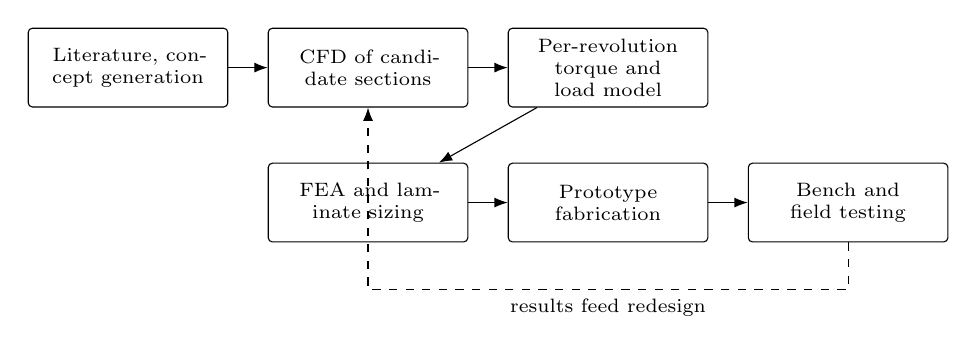
\begin{tikzpicture}[>=Latex,node distance=5mm,st/.style={draw,rounded corners=1.5pt,minimum height=10mm,text width=2.3cm,align=center,font=\scriptsize}]
 \node[st] (a) {Literature, concept generation};
 \node[st,right=of a] (b) {CFD of candidate sections};
 \node[st,right=of b] (c) {Per-revolution torque and load model};
 \node[st,below=7mm of c] (e) {Prototype fabrication};
 \node[st,left=of e] (d) {FEA and laminate sizing};
 \node[st,right=of e] (g) {Bench and field testing};
 \draw[->] (a)--(b); \draw[->] (b)--(c); \draw[->] (c)--(d); \draw[->] (d)--(e); \draw[->] (e)--(g);
 \draw[->,dashed] (g.south) |- ++(0,-6mm) -| (b.south) node[pos=0.25,below,font=\scriptsize]{results feed redesign};
\end{tikzpicture}
\caption{Development loop. The aerodynamic model drives both the blade selection and the structural loads.}\label{fig:loop}
\end{figure}
We compared three concept families, drag-based cupped, lift-based and hybrid lift--drag, and rotor-arm options against the roadside wake conditions. 2D and 3D CFD in ANSYS gave lift and drag at the angles of attack a blade sees over a full turn. Because a helical vertical-axis rotor can be reduced to its cross-section behaviour, we also built a per-revolution model that turns lift and drag into tangential force and torque for three blades 120\textdegree\ apart, plus the centrifugal load, and used it to estimate power and voltage at 2.25, 12 and 24\,m/s. The test rig is far smaller than the full-scale design, so the rotor was re-engineered for the rig. We built two variants, a lift-based baseline and a hybrid, so that the CFD hypothesis about multi-directional wind could be tested and not assumed. Loads from the model were applied in a SolidWorks static study of the most heavily loaded part, the hub, which we combined with flexural tests of laminate coupons to choose the number of plies.

\section{The Carbon-Fibre Rotor}\label{sec:cf}
\subsection{Why it was needed}
The first prototype, printed in PLA, proved the concept and exposed three limits that matter for a roadside machine: low stiffness for its mass, so the rotor stores little rotational energy and flexes in gusts; high mass, which raises the start-up wind speed; and, for UAE use, a polymer that softens near the temperatures of sun-baked surfaces. Typical PLA datasheet values (about 60\,MPa tensile strength and 3.5\,GPa modulus) are roughly an order of magnitude below those of carbon-fibre laminates, although the comparison is indicative only because our own coupons were loaded in bending, not in tension.

\subsection{Choosing the laminate: flexural tests and FEM}\label{sec:fem}
\textbf{Flexural tests.} In a materials laboratory we loaded rectangular coupons, about 22\,mm wide, to failure in bending and computed the flexural strength from the failure load and the section (\cref{fig:coupons}). Each group has five coupons (\cref{tab:flex}). Hand-laid carbon fibre is far stronger than the chopped-strand and woven-glass laminates tested alongside it, and strength rises with the number of plies in the hand-laid carbon coupons. Spread within each group is 5--8\%.
\begin{table}[t]\centering\small
\begin{tabular}{@{}llrr@{}}\toprule
Material & Process & Mean flexural strength (MPa) & Spread (\%)\\\midrule
Chopped-strand mat & hand layup & 214.9 & 7.9\\
Chopped-strand mat & vacuum infused & 261.4 & 7.0\\
Woven glass & hand layup & 395.8 & 6.0\\
Carbon, 4 plies & hand layup & 474.9 & 6.5\\
Carbon, 6 plies & hand layup & 596.7 & 4.8\\
Carbon & vacuum infused & 568.0 & 6.2\\\bottomrule
\end{tabular}
\caption{Flexural strength of laminate coupons, five specimens per row. Spread is the standard deviation as a percentage of the mean. These are coupon results, not the schedule of the rotor.}\label{tab:flex}
\end{table}
The strongest single coupon reached 644\,MPa. Six-ply hand layup matched or exceeded vacuum infusion in this set, which is consistent with our decision to work by hand layup alone, but the two groups differ in thickness and the test was not designed to separate the process from the ply count.

\textbf{Finite-element study.} The part that carries the most load is the hub, a three-armed plate that joins the rotor tube to the arms. We modelled it in SolidWorks as a static study with the loads from the aerodynamic model applied at the arm tips (\cref{fig:fem}). The peak von Mises stress was about 8.6\,MPa, under 2\% of the lowest carbon flexural strength in \cref{tab:flex}. A single-material static study does not resolve ply-level stresses, so we used it as an approximate value, and set the number of plies from this result together with the coupon data and with what the hand layup could produce reliably. The ply schedule is not published.
\begin{figure}[t]\centering
\begin{subfigure}{0.40\linewidth}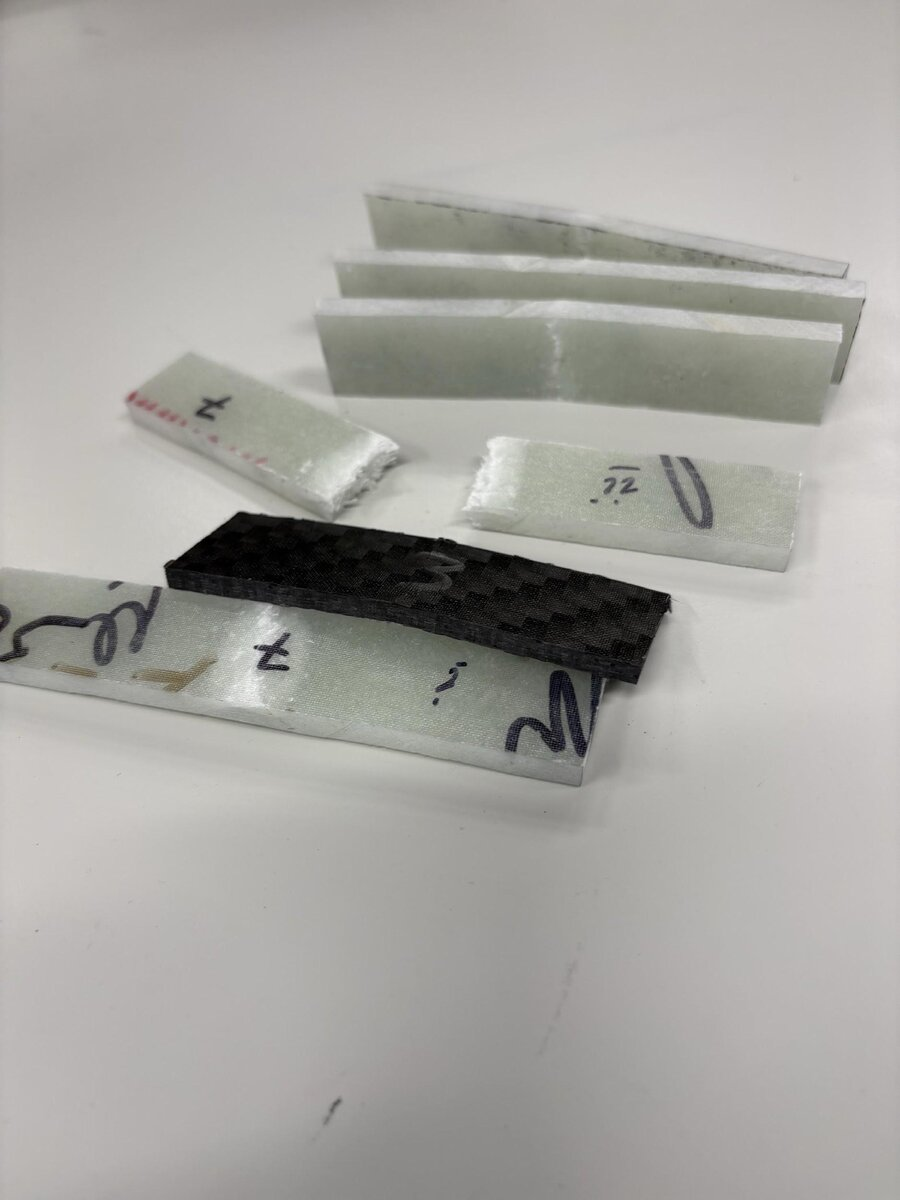
\includegraphics[width=\linewidth]{figures/coupons_photo.jpg}\caption{Coupons after bending tests.}\end{subfigure}\hfill
\begin{subfigure}{0.56\linewidth}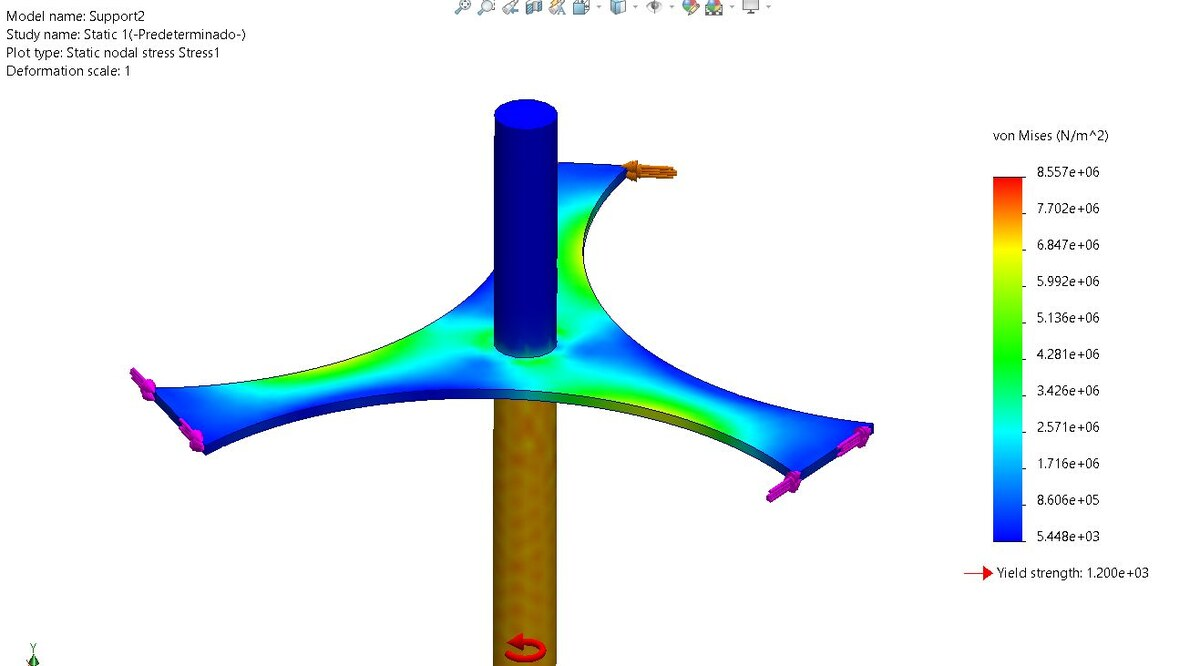
\includegraphics[width=\linewidth]{figures/hub_fem.jpg}\caption{Von Mises stress in the hub.}\end{subfigure}
\caption{Laminate coupons and the finite-element study of the hub.}\label{fig:coupons}\label{fig:fem}
\end{figure}

\subsection{What we built}
Every composite part is a hand layup.
\begin{itemize}
\item \textbf{Blades.} Woven carbon fabric and resin laid by hand into a single-piece, concave mould printed in PLA (\cref{fig:layup}).
\item \textbf{Central tube.} Carbon fabric wrapped under tension on a wooden mandrel covered with a Teflon sheet and a Mylar film, and cured at ambient temperature. The resin reached an exothermic peak of about 60--80\,\textdegree C.
\item \textbf{Hub.} A flat hand-laid laminate cut to a drawing, with the three arms of the FEM model.
\end{itemize}
\begin{figure}[t]\centering
\begin{subfigure}{0.48\linewidth}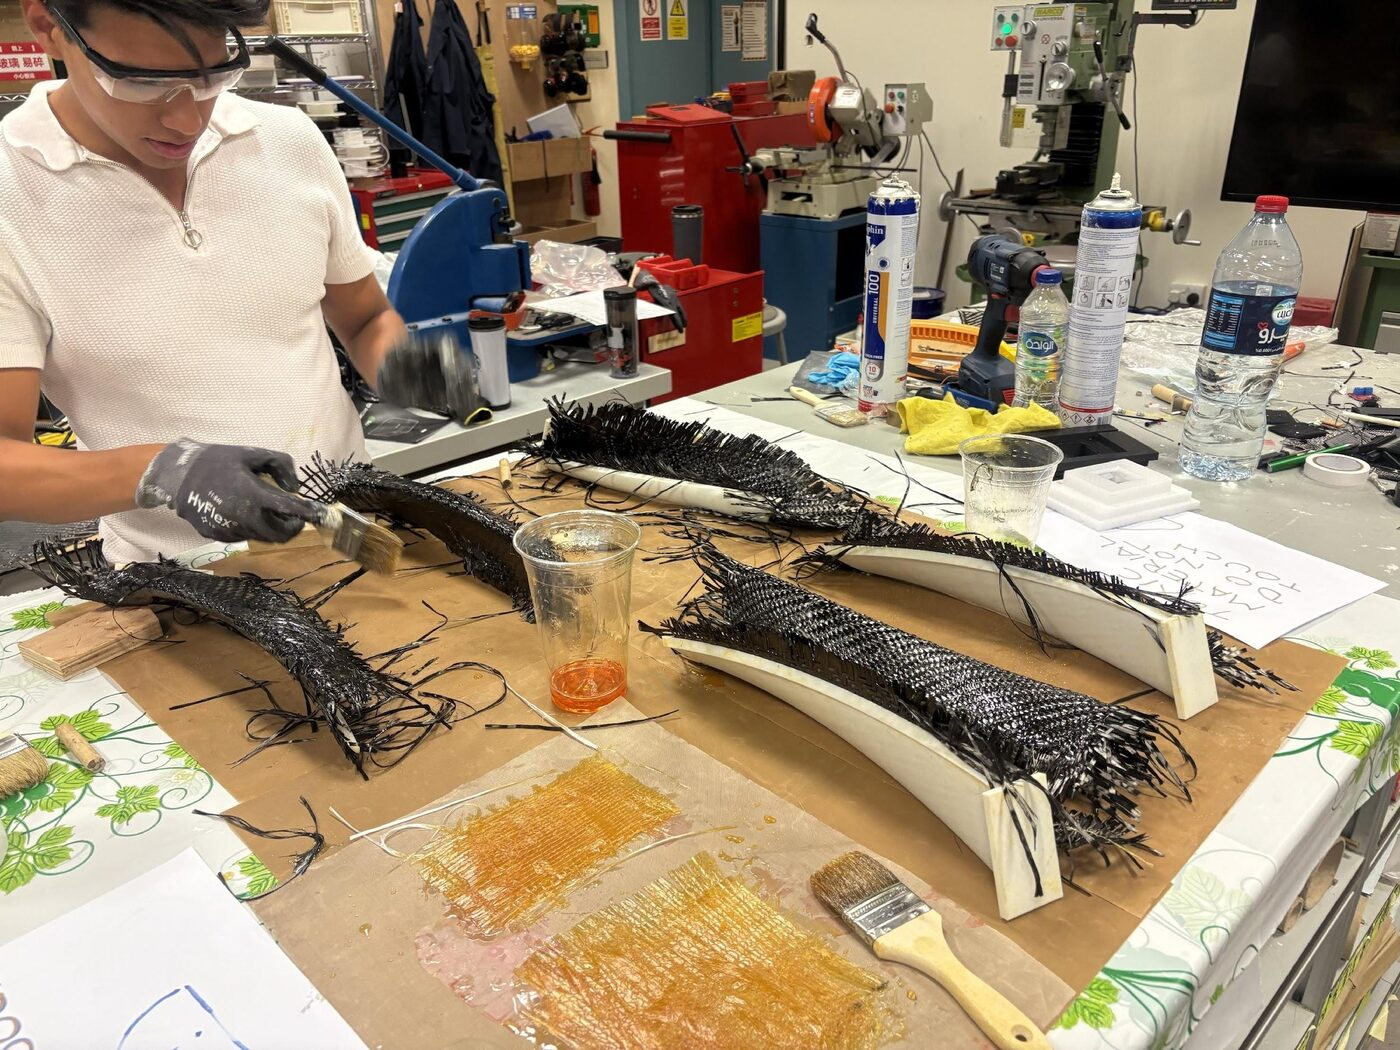
\includegraphics[width=\linewidth]{figures/blade_layup_1.jpg}\caption{Laying up the blades.}\end{subfigure}\hfill
\begin{subfigure}{0.48\linewidth}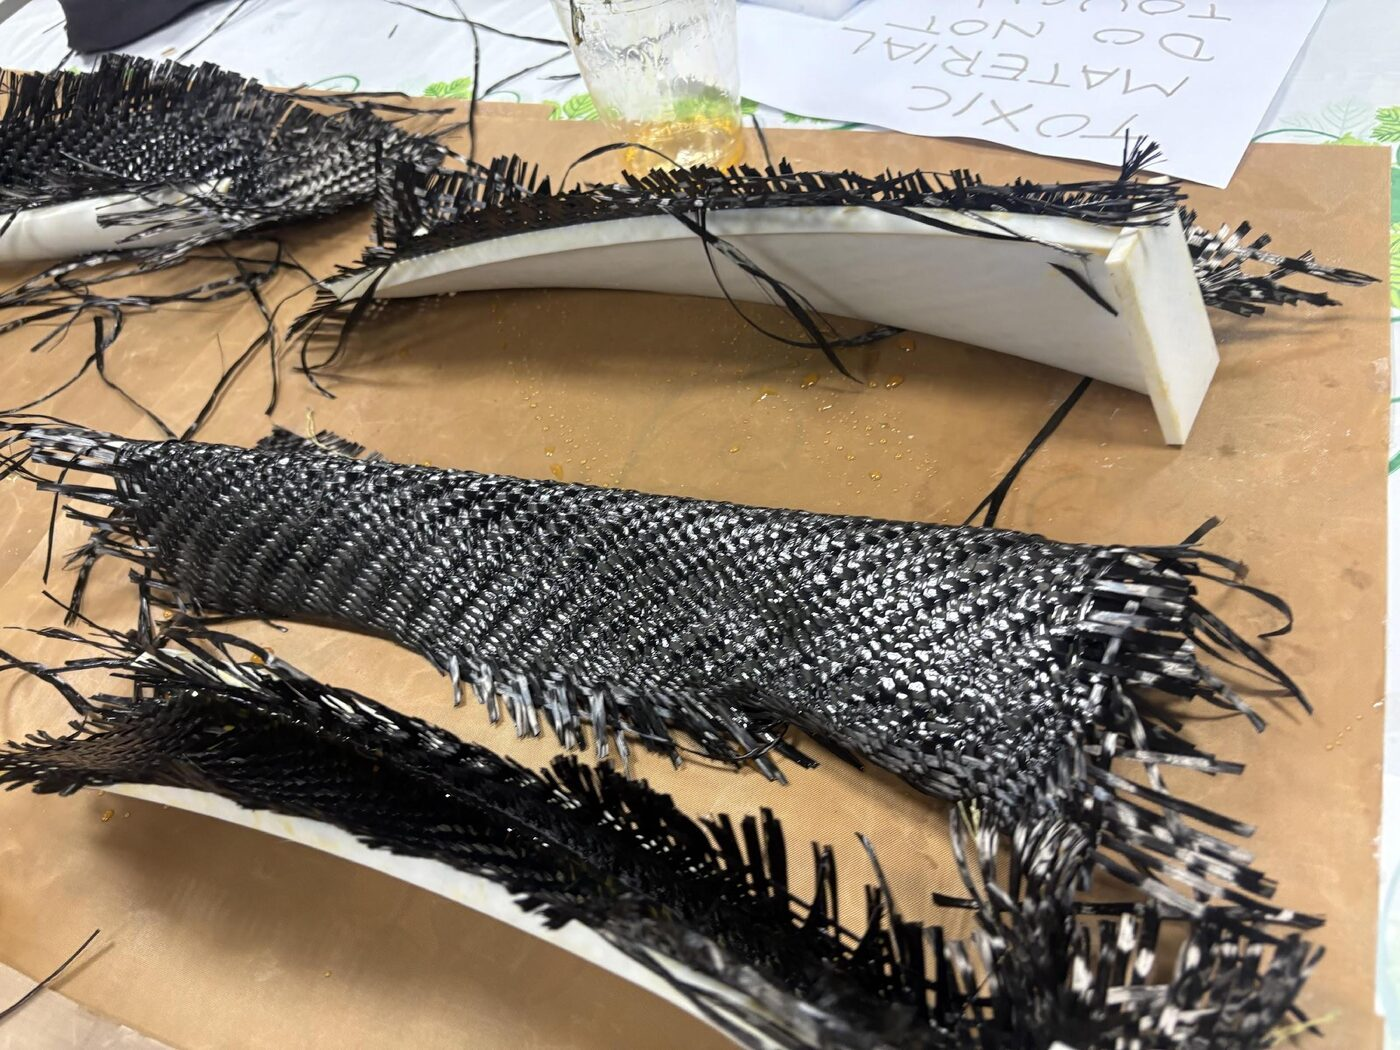
\includegraphics[width=\linewidth]{figures/blade_layup_2.jpg}\caption{Fabric on the printed moulds.}\end{subfigure}
\caption{Blade fabrication by hand layup.}\label{fig:layup}
\end{figure}

\subsection{What went wrong, and what we changed}
\textbf{Tube, first attempt.} The Teflon sheet was held with adhesive tape. The exotherm degraded the tape, which bonded to the laminate, and the tube could not be released. In the second attempt we removed the tape from the wetted region and put a continuous Mylar barrier layer under the fabric; the tube released cleanly. The lesson is that every release layer, and anything touching it, must survive the cure temperature.

\textbf{Blades.} A one-piece concave mould made the second half of each blade difficult to lay, and resin settled into the inner parts. Two-part moulds suit complex shapes better.

\textbf{Hub.} The first cutting layout left no room for the second arm. The cutting instructions have to state exactly what is cut and where, including the space needed for every arm.

\subsection{Scope of the claim}
The aim was a complete load path and not only a material swap: loads from our own aerodynamic model go into a finite-element study, and the result is combined with coupon tests to choose a laminate that can be made by hand with a student budget. In the literature we reviewed, small vertical-axis harvesters were typically printed or sheet-metal prototypes; we did not find a roadside traffic-wind harvester with an all-composite rotor built this way. This is a statement about our review and not a patent-search or priority claim.

\section{Instrumentation}\label{sec:daq}
All measurements come from a self-contained logger built around an Arduino Uno, an SD-card module and a resistive divider of 10\,k$\Omega$ and 2\,k$\Omega$, which scales a turbine voltage of up to about 29\,V into the 5\,V ADC range. It was calibrated against a known source to within $\pm$0.05\,V. A sample is written only when the voltage moves by more than 0.5\,mV, which filters noise and spares the SD card on hours-long runs. A zero entry is written every ten minutes so that a flat line can be told from a dead logger. A new file (\texttt{volt1.csv}, \texttt{volt2.csv}, \ldots) is created at every power-up, and time stamps are elapsed time since power-up because there is no real-time clock.

Unstable supply regulation and coupling between components initially corrupted the readings. We added voltage-regulation modules, shielded cables and isolated sensor channels, and housed everything in a painted box with an SD-card access compartment (\cref{fig:daq}). The logging sketch is in the repository under \texttt{daq/}.
\begin{figure}[t]\centering
\begin{subfigure}{0.40\linewidth}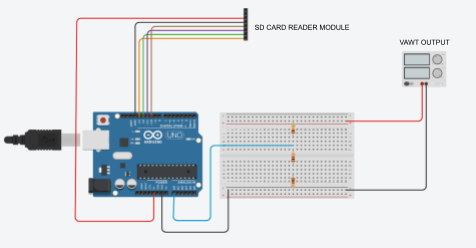
\includegraphics[width=\linewidth]{figures/daq_wiring.png}\caption{Logger schematic.}\end{subfigure}\hfill
\begin{subfigure}{0.27\linewidth}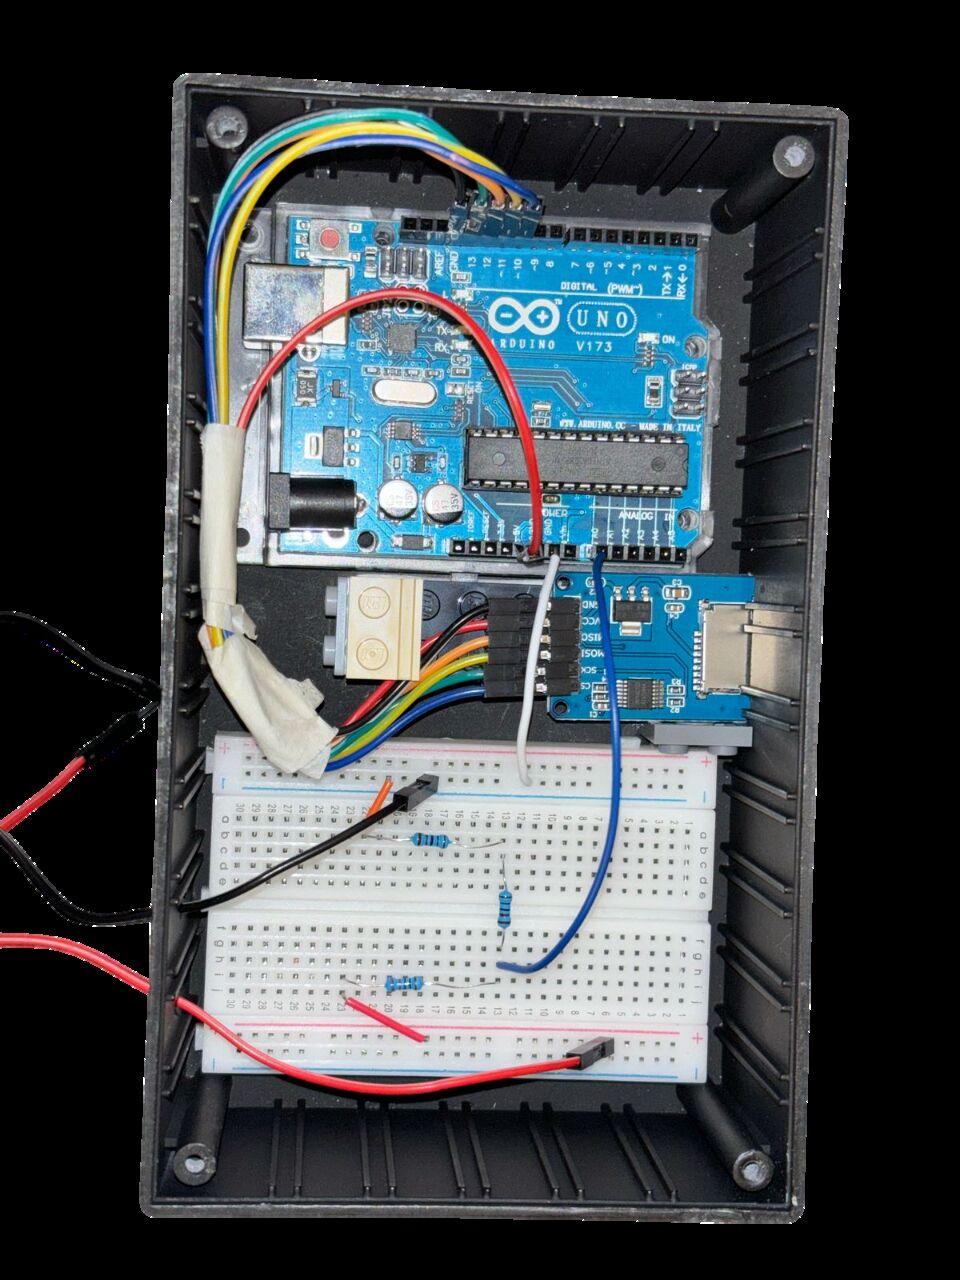
\includegraphics[width=\linewidth]{figures/box_inside.jpg}\caption{Inside the box.}\end{subfigure}\hfill
\begin{subfigure}{0.27\linewidth}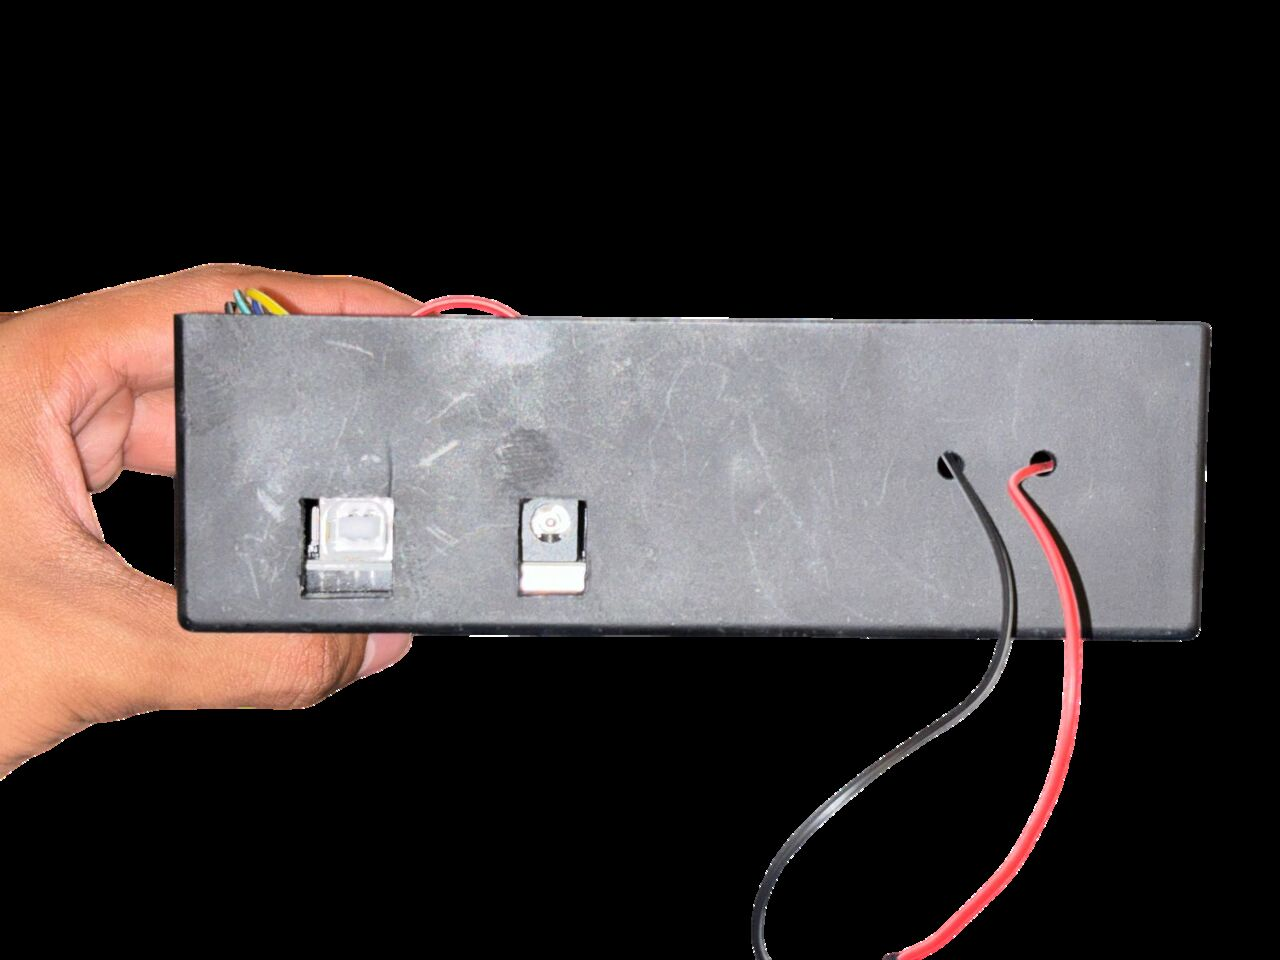
\includegraphics[width=\linewidth]{figures/box_front.jpg}\caption{Input panel.}\end{subfigure}
\caption{Data-acquisition system.}\label{fig:daq}
\end{figure}

\section{Tests and Results}\label{sec:results}
\subsection{Bench tests with a controlled fan}
A high-velocity fan one metre from the rotor held 6, 12 and 24\,m/s for 90\,s, after which the rotor coasted down with logging continued. \Cref{fig:typeA} and \cref{tab:typeA} give the output of the PLA prototype. Output rose clearly only at 24\,m/s, where the rotor also kept more momentum. At 6--12\,m/s it was low, which is the regime that matters at the roadside, and that finding drove the mass-reduction and composite work.
\begin{figure}[t]\centering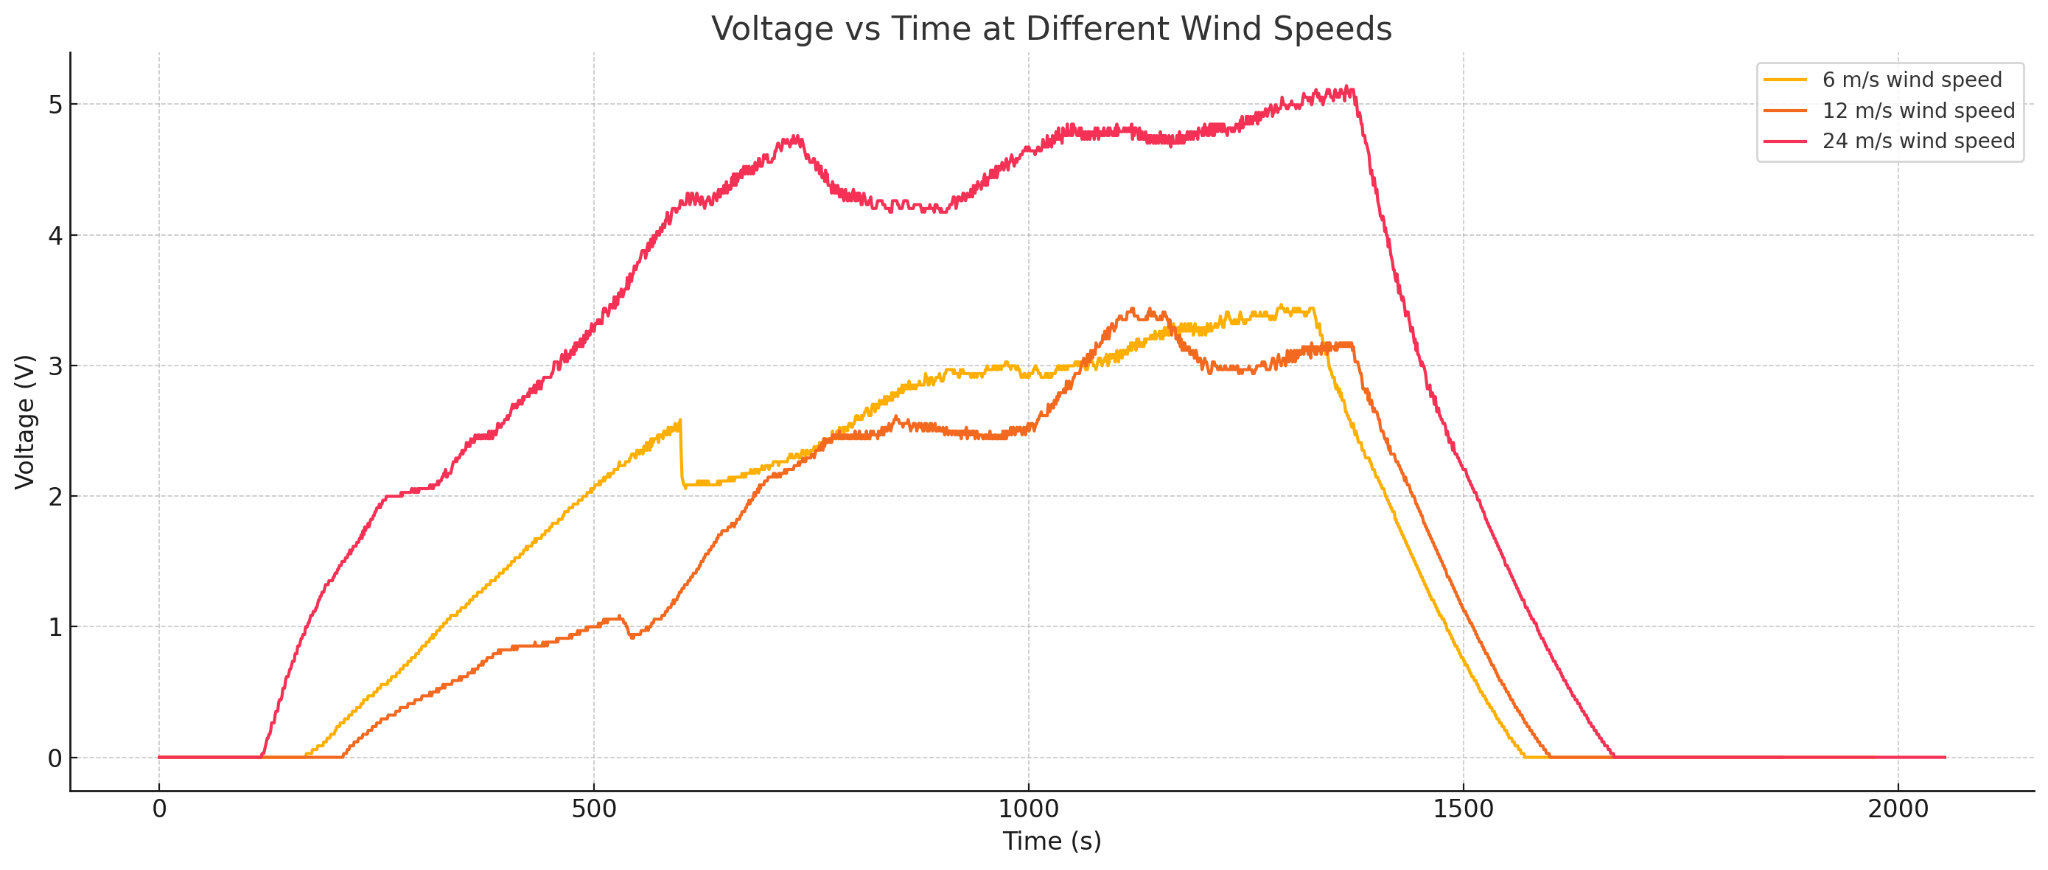
\includegraphics[width=0.8\linewidth]{figures/typeA_all.png}
\caption{Output of the first (PLA) prototype at three constant wind speeds.}\label{fig:typeA}
\end{figure}
\begin{table}[t]\centering\small
\begin{tabular}{@{}rrr@{}}\toprule
Wind speed & Average voltage (V) & Peak voltage (V)\\\midrule
6\,m/s & 1.53 & 3.47\\ 12\,m/s & 1.42 & 3.44\\ 24\,m/s & 2.59 & 5.14\\\bottomrule
\end{tabular}
\caption{Bench results, PLA prototype.}\label{tab:typeA}
\end{table}

\subsection{Field test}
The first on-street test ran on the bridge between Saadiyat Island and the NYUAD campus during busy hours, logging for 3\,h\,43\,min with a peak of 5.49\,V (\cref{fig:field}). Output was inconsistent in traffic, and after the first hour readings stayed below about 3.5\,V. Moving to a more exposed spot on campus raised readings by about 66\%, which shows how strongly siting affects a roadside harvester.
\begin{figure}[t]\centering
\begin{subfigure}{0.28\linewidth}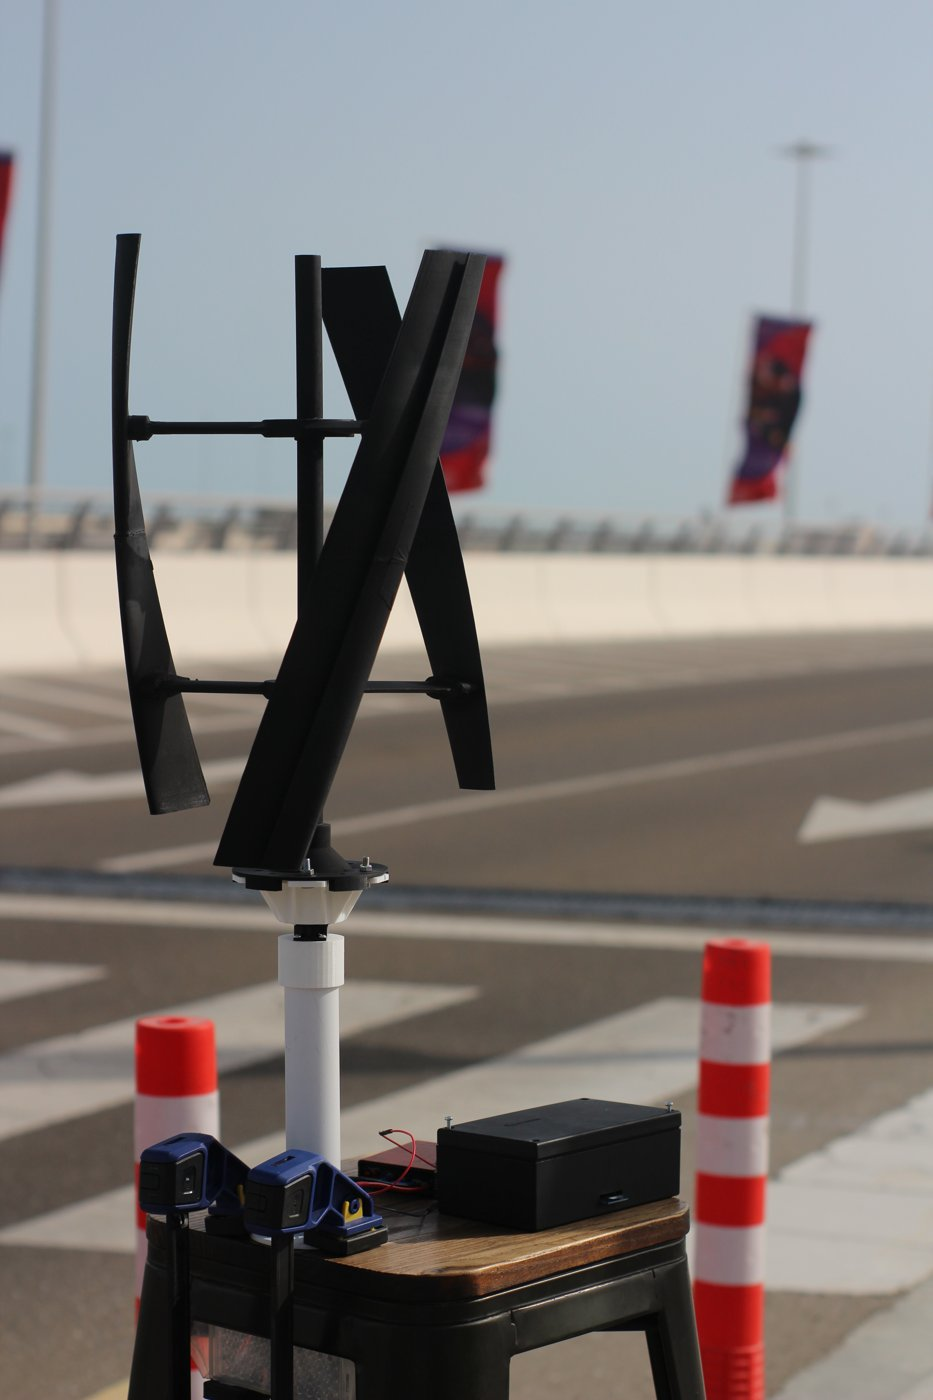
\includegraphics[width=\linewidth]{figures/field_test_1.jpg}\caption{Test stand and logger at the roadside.}\end{subfigure}\hfill
\begin{subfigure}{0.66\linewidth}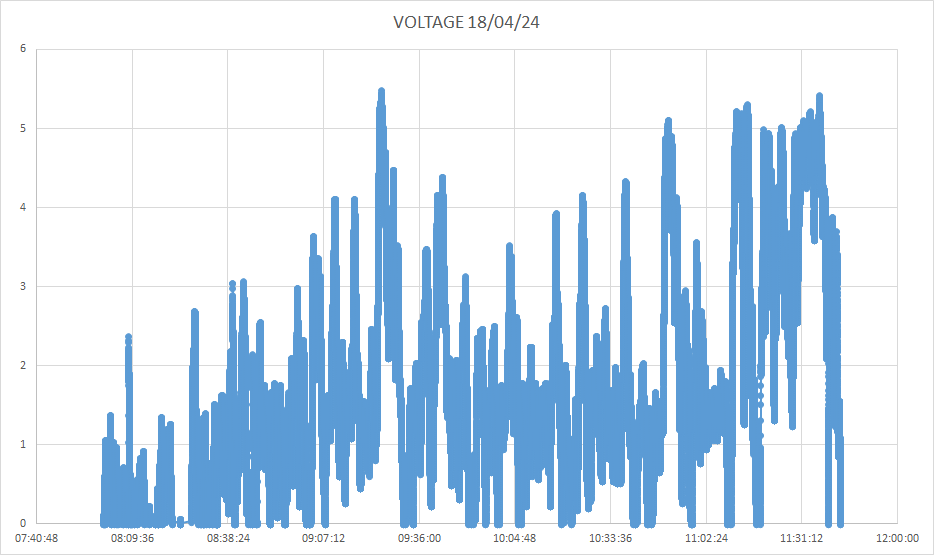
\includegraphics[width=\linewidth]{figures/field_pla.png}\caption{Voltage record, PLA prototype.}\end{subfigure}
\caption{Field test, April 2025.}\label{fig:field}
\end{figure}

\subsection{PLA against carbon fibre}
\begin{figure}[t]\centering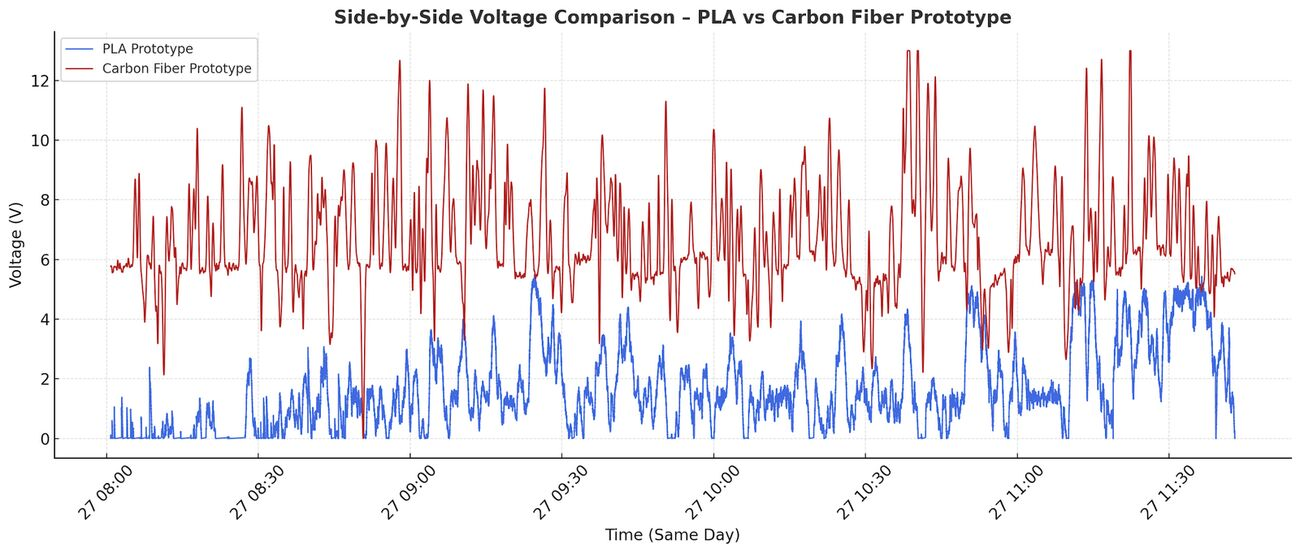
\includegraphics[width=0.88\linewidth]{figures/pla_vs_cf.jpg}
\caption{Voltage records of the PLA prototype (blue) and the carbon-fibre prototype (red). The common time axis is synthetic: the two records come from separate sessions and are aligned for comparison.}\label{fig:plavscf}
\end{figure}
\begin{table}[t]\centering\small
\begin{tabular}{@{}lrr@{}}\toprule
Metric & PLA prototype & Carbon-fibre prototype\\\midrule
Mean voltage (V) & $\sim$2.1 & $\sim$6.8\\
Maximum voltage (V) & 5.49 & 13.02\\
Minimum voltage (V) & 0.0 & $\sim$1.4\\
Standard deviation (V) & $\sim$1.26 & $\sim$2.9\\
Share of record above 2\,V & $\sim$42\% & $\sim$88\%\\\bottomrule
\end{tabular}
\caption{Statistics of the two field records.}\label{tab:plavscf}
\end{table}
The gain is large and consistent across the record (\cref{fig:plavscf,tab:plavscf}). The mass reduction of about 60\% in the rotor arms relative to the printed ones is an estimate from the analysis and not a weighing.

\subsection{Status against the requirements}
\begin{table}[t]\centering\small
\begin{tabular}{@{}p{1.7in}p{3.2in}@{}}\toprule
Requirement & Status\\\midrule
Energy conversion $\ge20\%$ & Partly shown at high wind speed; not shown at 6--12\,m/s. Load-based power measurement still needed.\\
Fatigue, $10^7$ cycles & Not tested; analysis only.\\
Noise below 45\,dB(A) at 10\,m & Not measured.\\
60\,\textdegree C and UV & Composite chosen for this reason; accelerated ageing not run.\\
Yaw or adaptive control within 500\,ms & Concept only.\\
Maintenance and cost & Sealed bearings and coatings specified; not field-proven.\\\bottomrule
\end{tabular}
\caption{Status against the design targets.}\label{tab:status}
\end{table}
The prototype budget was about 1\,670\,AED (roughly US\$450), including the carbon fabric, resin and release layers.

\section{Discussion}\label{sec:discussion}
\textbf{Practical consequences.} At the low wind speeds that matter at the roadside, mass and start-up behaviour dominate, and siting changes the output as much as the rotor does. We would take the composite route as the baseline for deployment.

\textbf{What this study does not establish.} The records are output voltages through one divider and logger, not electrical power. The PLA and carbon-fibre records come from separate sessions under different wind, so the 3.2-fold ratio is an observation and not a controlled comparison. The 60\% arm-mass saving is an estimate. The coupon tests compare processes that differ in thickness and ply count, and the hub study is a single-material approximation. The published logging sketch differs from the one used for the records in its file naming and elapsed-time stamps, and has not been re-run on the rig. We have not measured power with a resistive load, run a like-for-like wind-tunnel test, tested fatigue to $10^7$ cycles or any aspect of long-term durability, measured noise, aged the material under UV and 60\,\textdegree C, or built the yaw control.

\textbf{Next steps.} Validate power and energy with a resistive load; run a like-for-like wind-tunnel test of the PLA and composite rotors; reduce rotating mass and bearing friction to lower the cut-in speed; and add the environmental, fatigue and acoustic tests above.

\textbf{Conclusion.} A hand-laid carbon-fibre rotor is practical on a capstone budget and, in our records, produced about three times the mean voltage of the printed rotor and stayed above 2\,V for most of the record. The measurement is a voltage and the sessions differ, so the next step is a controlled power test, and the design targets for efficiency, fatigue, noise and ageing remain open.

\section*{Acknowledgements}
We thank our supervisors Pradeep George, Jeremy Teo and Je Ir Ryu; Jorge Montalvo for manufacturing support; Khaled Shahin for advice on composites and mechanics of materials; and the NYUAD Engineering Division.

\section*{Code and data availability}
The logging sketch and the report source are in the repository accompanying it. Aerodynamic definitions, dimensions and laminate schedules are not published.

\bibliographystyle{plainnat}
\bibliography{references}
\end{document}
